%% ----------------------------------------------- %%
%%            Graphical user interface             %%
%% (documentation chapter for the FilmTit project) %%
%% ----------------------------------------------- %%

\section{Goals}
% (Honza)
Our main goal is to offer a tool for the translators of the movie subtitles as easy and effective to use as possible. With the capabilities of the current web browsers, we decided to make FilmTit a web-based application, therefore sparing the user the need to download and install anything.

\section{Google Web Toolkit}
% (Honza and Ruda)
The web-based user interface representing the client part of the FilmTit application is based on the Google Web Toolkit (GWT) framework. This technology is a development toolkit for building and optimizing browser-based applications %\citep{Gwtweb}
and is based on the idea of translation of Java source code into Javascript. Therefore, it enables us to write in Java even on the client side, but preserving most of the advantages of web application accessibility for the user.

The official description of GWT isas follows:

Google Web Toolkit (GWT) is a development toolkit for building and optimizing complex browser-based applications. Its goal is to enable productive development of high-performance web applications without the developer having to be an expert in browser quirks, XMLHttpRequest, and JavaScript. GWT is used by many products at Google, including Google Wave and the new version of AdWords. It's open source, completely free, and used by thousands of developers around the world.

We decided to use GWT for several reasons.

One reason is that it integrates very well with the rest of the application, which is written in Java. A prominent example is the communication between GUI and Userspace. Not only is the interface defined by one simple Java class (FilmTitService.java), which is then used both by the GUI and the Userspace, but thanks to GWT we are even able to use exactly the same classes (placed in share) in GUI and in Userspace and send them easily through the FilmTitService interface. Thus, we avoided the trouble of having to keep each of these classes in two versions, Java and Javascript, together with mappings to and from the transport format. In fact, all of these do exist in the application, but only in the compiled code, completely hidden from the developer.

However, there is a downside which can be expected but is difficult to manage properly. It is obvious that GWT does not support everything that exists in Java -- instead, it supports only a subset of Java, with a lot of GWT-specific additions. This is perfectly reasonable, and, as the subset supported is large enough, should not cause any problems. However, the cut between supported and unsupported features is very misty -- often a class is supported (e.g. LinkedList), but only some of its methods are implemented (e.g. one can use removeFirst(), but pop() is unsupported). Moreover, the IDE does not provide much support in this area, so often the only thing that a developer can rely on are internet forums. Luckily, GWT is used by many developers and most of the issues that we encountered had been already solved by others. Still, we spent a lot of debugging time on problems that were actually problems of GWT that had to be worked around, instead of being problems of our code.

A requirement that we had for the web technology was to offer an IDE (in GWT realized by a plugin for Eclipse IDE, similarly applicable also for IntelliJ IDE), possibly with debugging support. In GWT, there is a dedicated Development Mode for these debugging purposes, sparing the developer the need of recompiling all the GWT code for testing after each change. This proved to be very efficient in the first phases of the development when the GUI module was developed independently and although it turned out to be quite difficult to set up once this module was integrated with the rest of the project, it remained one of the most useful features of GWT.

Another option that we found useful is the possibility to directly insert real Javascript code into GWT methods. Although it is not very clean and cannot benefit from some of the features of GWT, it is sometimes the only way how to do something that is supported in Javascript but unsupported in GWT.

An important point also was that GWT is freeware (it is even open-source, but we did not benefit from it much), or more precisely, is licensed under the Apache License, v.~2.0 (TODO: citation for the license!), with several third-party software included in its distribution under other freeware licenses.

Although GWT can be integrated into a Maven project, it was far from flawless and a lot of time had to be spent on making everything work together, including maintaining the IDE support. We managed to do that in the end, but we had expected this to be much easier. The main reason (but not the only one) is the specific directory structure, different for the Maven project and for the GWT project, which has to be adjusted in the configuration of both the Maven plugins and the IDE.

To conclude, we are happy that we decided to use GWT because of the benefits it brought to us, but we were disappointed by the number of complications that it brought as well. Were we to decide on a web framework to use for a similar project, we would still have to consider our decision carefully.

\subsection{Browser Support and Optimization}
GWT also provides a feature which makes the final web application similar in different major browsers and optimized to a certain degree for each of them. This feature is called {\em deferred binding} and it is based on generating different versions of the Javascript code during compile time, only one of which needs to be loaded by a particular client browser at runtime. This process is by default maintained by the GWT compiler itself, so that the developer does not have to worry about it.

However, this ``unification'' is not complete, nor it is intended to be. It covers only the bigger and more crucial differences of the code behaviour among various browsers, but does not address some slight variancies e.g. in design of the basic elements (and their most common behaviour). This seems reasonable, because forcing each browser to interpret the code in the exact same way would mean hardcoding almost everything from scratch and not using many of their provided features, which would be probably impossible anyway. Nevertheless, some of these ``slight differences'' which we have encountered proved to be quite crucial for our intended design (especially in the event-handling domain), so lots of work had to be done to reasonably unify the application's behaviour even among the major browsers.

Still, our hope is that GWT development will continue and will keep up with the development of web browsers, allowing us to provide browser-up-to-date versions of FilmTit simply by acquiring a new version of GWT and recompiling the project.

TODO: FilmTit actual browser support -- tested and optimized for what? (here or somewhere else?)

\subsection{Designing by UiBinder}
Another very useful and comfortable feature of the GWT for designing the user interface is the UiBinder. The idea behind this approach is to design the visual structure of the page (or its part) in an HTML-like way (this is called the {\em UiBinder template}) and its behaviour and functionality in a Java class (called the {\em owner class} for the template). The UiBinder itself is then an object binding these two approaches together. This style of creating the web application supports the respected best practice to divide the visual design and the functionality. It also allows to create the web page's appearance in a way which is more natural to web designers (e.g. HTML-like), as well as more readable and modifiable. Other advantages includes supposedly better performance (as the browsers can better optimize the rendering from the UiBinder templates than from the heavier-weight Java-based widgets and panels) and support for internationalization (not used by FilmTit at the moment).

The actual source code of a page designed this way (or of its segment) then consists of a file with the *.ui.xml Ui-Binder template (where also the style definition can be included directly) and a corresponding *.java owner class, where the elements of the template can be accessed as widgets (as well as made accessible to other classes). The owner class then can be simply instantiated and plugged into an existing design just like any other widget.

\subsection{Twitter Bootstrap Library}
For enhancing the visual appearance of our application to a modern look without a professional graphic designer, we have decided to use an existing open-source library for GWT which displays the page elements (and their groups) in the style of the Twitter pages. This library is called GWT-Bootstrap and is easily applicable with the UiBinder-style designing. It is also still a live project, so there is a hope that more features would be available in the possible future development.

Similarly to other third-party libraries used by FilmTit, the GWT-Bootstrap library is attached as a Maven dependency and downloaded automatically from its own Maven repository.


\section{GUI Structure}
% (Honza/Ruda)

(I am not sure what this section should look like, so I'm just drafting something.... RR)

The main class is Gui.java. It defines the web application itself, providing an entry point and initialization methods. It also handles general requests.

FilmTitServiceHandler.java provides wrappers for the ``raw'' RPC calls. It offers methods with names and parameters similar to the actual RPC methods, also providing response and error handling.

An important class is the SubgestBox, or ``SUBtitle sugGESTion BOX'', which visualizes the TM results, offering a variety of means of navigation through them.

Some settings have to be done via several resource files in the webapp directory. (This is required by the Java Servlets technology used to deploy the application.) Don't forget to refer to the sitemap figure \ref{fig:sitemap}.

\begin{figure}
\begin{center}
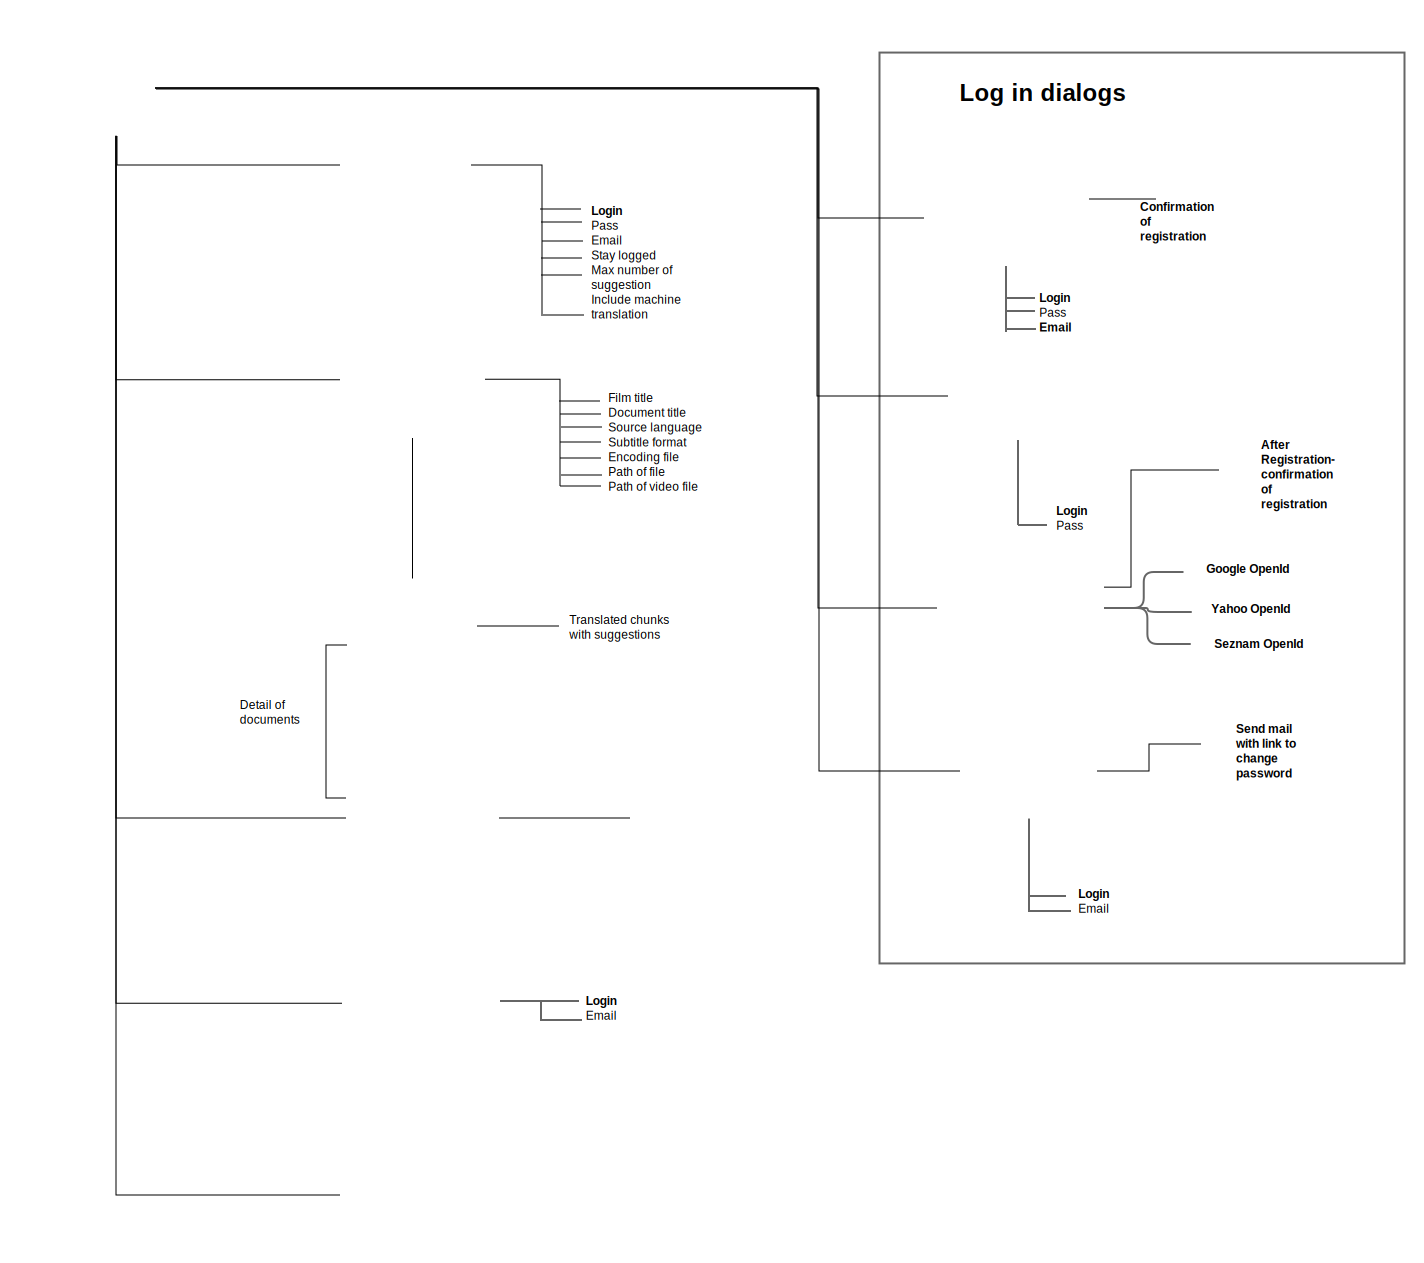
\includegraphics[scale=0.4]{figures/sitemap.pdf}
\end{center}
\caption{Site map of the application}
\label{fig:sitemap}
\end{figure}

\subsection{Parsing and segmentation}
% (maybe Karel?)


\section{Communication}
\label{sec:communication}
\subsection{RPC}
% (Ruda)

\subsection{Communication Scheme}
GUI communicates with Userspace via a GWT RemoteService implementation, defined as the FilmTitService interface.
The interface provides asynchronous RPC methods (the responses are processed by callbacks).

The method is always called from the client, because Javascript security policies do not allow to handle incoming calls.
Therefore, in case the Userspace needs to actively contact the GUI without the GUI having sent a request before,
this has to be implemented in the GUI by polling.

\subsection{Manipulating the documents}

\subsubsection{createDocument}
	Document createDocument(String movieTitle, String year, String language);

Userspace creates a Document instance with the given title, year and language.
It checks the data with IMDB and fills in other information if a corresponding movie is found.
Once the Document is created, it is sent back to the GUI.

\subsubsection{getTranslationResults}
	TranslationResult getTranslationResults(TimedChunk chunk);
	
Userspace passes the given chunk to the core, which generates zero or more translation suggestions.
These are packed into a TranslationResult instance and sent back to GUI.

\begin{figure}[h]
\begin{center}
\includegraphics[scale=0.45]{figures/document_creation_sequence.pdf}
\end{center}
\caption{Sequence diagram of document creation, including translation suggestions loading.}\label{gui:sd:document_creation}
\end{figure}

\subsubsection{setUserTranslation}
	Void setUserTranslation(int chunkId, long documentId, String userTranslation, long chosenTranslationPair);

This method is called once the user selects a suggested translation and optionally post-edits it
(or does not select one but inputs the translation text directly).
The translation is then saved by Userspace;
the id of the TranslationPair chosen for post-editing is also sent, providing feedback which then can be used to improve future suggestions.

\subsection{User login}

The user is required to log in to be able to save his work on the server.
TODO: Do we allow the user to work without being logged in?

The user is logged in if he has a valid session id which is linked to a user account in Userspace.
The session id expires after a given period of time without any user interaction with the server,
it is therefore neccessary that the user can log in without the application\'s main window being reloaded so that the user does not lose unsaved data.

\subsubsection{Simple Login}
\label{subsec:simple_login}

TODO: There is simple login which is very simple. See Figure \ref{gui:sd:simple_login}.


\begin{figure}[h]
\begin{center}
\includegraphics[scale=0.65]{figures/simple_login_sequence.pdf}
\end{center}
\caption{Sequence diagram of simple login and logout.}\label{gui:sd:simple_login}
\end{figure}

\subsubsection{Login via OpenID Services}
\label{subsubsec:gui_openid}

The authentication itself is done in a new authentication window.
A successful authentication is then paired with the GUI instance using a temporary one-time identifier, authID, shared by the main window and the authentication window.
(Because of Javascript security restrictions, there is no simple way of sending the result of the authentication process from the authentication window to the main window;
however, it is straightforward to generate the authID in the main window, store it in Userspace and send it to the authentication window on its creation.)

When the main window requests user authentication, it generates the authID, calls getAuthenticationURL and opens an authentication window with the returned URL.
Then it waits for the user to authenticate in the authentication window
-- the waiting is active, polling the Userspace with getSessionID in regular intervals.
TODO: I suggest every 3 seconds for the first 2 minutes, then every 10 seconds for the following 8 minutes, and then every 30 seconds forever.
And, of course, if the main window regains focus, we call getSessionID immediately.
For each of the authentication services, there is a webpage that enables the user to authenticate
(its URL is returned by getAuthenticationURL)
and then passes information about the result of the authentication to a webpage given to it as a get parameter
(we use the Authentication Response Window as the target webpage).
The result is then sent to Userspace by validateAuthentication.
If the authentication is successful, a new session is created for the user.
The main window then acquires the new session id via getSessionID and the authentication process is completed.

Several ways of authenticating the user are supported, including authentication by Google openID and Facebook account.

\subsubsection{getAuthenticationURL}
    String getAuthenticationURL(long authID, AuthenticationServiceType serviceType);

Called by GUI when authentication is required and the user is not logged in (i.e. does not have a valid sesion id).
A temporary one-time identifier, authID, is generated for the authentification session only to identify the client logging in and sent to Userspace together with the request.
The chosen service to be used for authentication is also given (e.g. Google or Facebook).
The Userspace returns a URL of the webpage to be used for authentication.

\subsubsection{validateAuthentication}
    Boolean validateAuthentication(long authID, String responseURL);

Called from the authentication response window after the user\'s attempt to authenticate themself.
The responseURL contains information from the authentication service to be checked and used by the Userspace.
If the authentication is found to have been successful, a new session is generated for the user and paired with the given authID, and true is returned.
Otherwise, the method returns false.

\subsubsection{getSessionID}
    String getSessionID(long authID);

Userspace checks whether a successful authentication has been done with the given authID.
If yes, the corresponding session id is returned.
Otherwise, null is returned.
TODO null or empty string?
TODO we still need to be able to send info that the user decided to cancel the authentication if we find this out - probably by an exception?

\begin{figure}[h]
\begin{center}
\includegraphics[scale=0.55, angle=90]{figures/openid_login_sequence.pdf}
\end{center}
\caption{Sequence diagram of OpenID login.}\label{gui:sd:openid_login}
\end{figure}

\section{Typical Usage}
% (Honza)
In the most typical case, a new user (already registered) will open the page with FilmTit and log in. Then, a dialog appears to create a new document corresponding to one movie, or more precisely, one subtitle file being translated from one language to another. Within this dialog, the user should specify which movie it is (title and year), what language pair will the translation be operating upon (e.g. from English to Czech) and provide the actual local file with the source subtitles (or alternatively, the user can paste the subtitles in appropriate format into a text-area). These information are sent to the Userspace and after refining the movie specification, the new document is created and the "translation working space" is filled with source subtitles (segmented to so-called "chunks") on the left side (as well as their timing) and corresponding empty text-boxes on the right side.

At the same time, the subtitle chunks are sent through the Userspace to the Core, where the appropriate suggestions are generated for them and sent back. When received in the GUI, the suggestions are displayed as some kind of suggest-box, or pop-up to the corresponding text-box for the given chunk, and sorted according to their supposed accuracy (still TODO). The user can then choose any one of them (or none) and edit it (if necessary) to get the desired translation of the particular chunk. When the user leaves the chunk to the next one, his translation is sent to the Userspace to be saved here as an intermediate translation of this chunk (???also to the Core???).

(still TODO:)
When finished with this chunk-after-chunk translation, the whole document is saved and processed as finished (sent to Userspace, Core etc.) and can be exported as a new subtitle file created from the (non-empty) translations.

\section{Video Playback}

TODO \todo{Karel should proudly describe what he did}
